%%%%%%%%%%%%%%%%%%%%%%%%%%%%%%%%%%%%%%%%%%%%%%%%%%%%%%%%%%%%%%%%%%%%%%%
% Based on IEEE the conference template available                     %
% at https://www.ieee.org/conferences/publishing/templates.html       %
% Adapted for the Data Science Lab course at Politecnico di Torino    %
% by Giuseppe Attanasio, Flavio Giobergia                             %
% 2020, DataBase and Data Mining Group                                %
%%%%%%%%%%%%%%%%%%%%%%%%%%%%%%%%%%%%%%%%%%%%%%%%%%%%%%%%%%%%%%%%%%%%%%%

\documentclass[conference]{IEEEtran}
\usepackage{cite}
\usepackage{amsmath,amssymb,amsfonts}
\usepackage{algorithmic}
\usepackage{graphicx}
\usepackage{textcomp}
\usepackage{xcolor}

\begin{document}

%\title{Predicting position of an electron using multioutput random forest regression}
\title{Prediction of particle position passing through a sensor with multiple readings}

\author{\IEEEauthorblockN{Michele Moneta, Alex Vellone}
\IEEEauthorblockA{\textit{Politecnico di Torino} \\
Student id: s317492, s331792 \\
\{s317492, s331792\}@studenti.polito.it}
}

\maketitle

%\begin{abstract}
%The paper shows an approach used in order to choose between a regressor or a classifier, so to %predict  the position of an electron passing though a RSD sensor.
%\end{abstract}

\begin{abstract}
This report presents a data science pipeline using scikit-learn Random Forest Regressor to 
predict particle positions based on multiple signals measured by a Resistive Silicon Detector.
\end{abstract}

\section{Problem overview}
In the particle physics field, the detection of the position of a particle is something physicists face continuously. 

%This is done with sensors, and in this specific case a \textit{RSD(Resistive Silicon Detector)} was used.The detector has a 2-dimensional surface with 12 metallic pads arranged in a snowflake-like pattern. When a particle passes through the sensor, it generates a signal(this in called an \textit{event}). Here a graphical representation of it: 

%In the domain of particle physics, the challenge at hand involves the precise detection of particle positions during their trajectories. Specifically, this project focuses on utilizing the Resistive Silicon Detector (RSD), a sensor with a 2-dimensional surface featuring distinctive "snowflake" shaped metallic pads. When a particle traverses the sensor, signals are generated by these pads, forming the basis for predicting the particle's (x, y) coordinates. 

This can be done with various types of sensors. In this specific case a \textit{RSD (Resistive Silicon Detector)} 
was used. This type of sensor has a 2-dimensional surface within which it can detect the passage of particles.
The RSD sensor has 12 “snowflake” shaped metallic pads that are used to measure \textit{signals}. 
When a particle traverses the sensor, signals are generated by these pads, forming the basis for predicting 
the particle's (x, y) coordinates.

For every signal measured by the pads we can extract some features:
\begin{itemize}
    \item pmax (positive peak magnitude): the magnitude of the positive peak of the signal, measured in millivolts (mV). 
    This represents the maximum amplitude of the positive part of the signal.
    \item negpmax (negative peak magnitude): the magnitude of the negative peak of the signal, measured in millivolts (mV). 
    This represents the maximum amplitude of the negative part of the signal.
    \item tmax (delay of positive peak): the delay, measured in nanoseconds (ns), from a reference time to when the positive peak of the signal occurs. 
    This indicates the time at which the peak of the positive signal is reached.
    \item area (area under the signal): the area under the signal curve.
    This provides information about the total charge or energy deposited by the particle as it passes through the detector.
    \item rms (root mean square): the rms value of the signal.
\end{itemize}

Figure \ref{fig:sensor_reading} shows a representation of a signal measured by a pad with all the features 
that can be extracted from it.\\
\begin{figure}[htbp]
\centerline{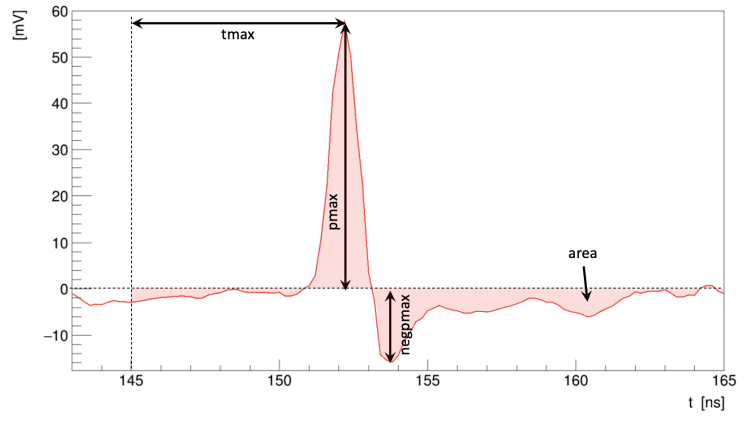
\includegraphics[width=\linewidth]{media/sensor_signal.png}}
\caption{Signal measured by a pad of the sensor.}
\label{fig:sensor_reading}
\end{figure}

The sensor output contains 18 readings of the event. Since only 12 pads are available, some of the 
readings are noise and does not contain actual readings.

The dataset contains 514,000 events, each providing 18 readings from the 12 pads. 
For each event the passage of a particle has been enforced (i.e. the (x,y) coordinates are known) and are available in the dataset.

This multi-output regression problem involves predicting the (x, y) coordinates of particles as they 
pass through a Resistive Silicon Detector (RSD), using the provided (x, y) coordinates and the 
pads readings as the evaluation set. 
The task requires analyzing the dataset and developing a data science pipeline to forecast particle 
coordinates from sensor readings, utilizing insights gained from the training dataset.


\section{Proposed approach}
TODO

You can use citations as follows: \cite{goodfellow2016deep} (you can add BibTeX citations in the \textit{bibliography.bib} file).


\subsection{Preprocessing}
User
In this phase we try to better understand the dataset, and try to manipulate it in order to prepare  for a deeper analysis  and the application of machine learning algorithms for classification or regression tasks.The dataset comprises 514,000 events, distributed into 385,500 instances for the development set(training and test set) and 128,500 for evaluation. The whole data collection comprises:

 514,000 rows, each referred to an event(also considering evaluation ones)
 
 92 columns, each for the indexed signal parameters extracted from RSD sensor

There are 18 indexed signal parameters  due to acquisition constraints, where 6 plus do not contain actual readings but rather noise.
Both x and y columns in development dataset contain 81 distinct values ranging in a discretized way from 200 to 600 um.
Below the grid representation: 

\begin{figure}[htbp]
\centerline{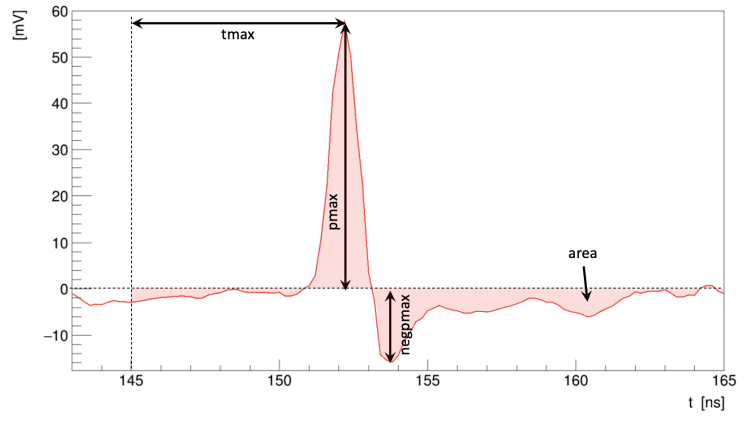
\includegraphics[width=\linewidth]{media/sensor_signal.png}}
\caption{Example of a figure caption.}
\label{fig2}
\end{figure}

The graphical representation of the dataset reveals a subarea, with overlapping points attributable to the controlled setting;the visual "holes" denote the positions of metallic pads on the sensor.
Specific outlier detection was omitted, given the perceived scarcity of outliers.
The train-test-split function from the Scikit-learn library facilitated development dataset division into training and testing sets. Initially, a 75-25\% split yielded 366,225 training values and 19,275 testing values. Subsequently, a 95-5\% split was employed for the final submission to enhance algorithm training.

 
\subsection{Model selection}
 
The criterion adopted for assessing the selection of the optimal predictive model in terms of prediction accuracy was the mean Euclidean distance between the obtained predictions and the target values.

Initially, a decision tree classifier was employed. This choice was motivated by the limited number of classes, the inherent efficiency of this model, and its versatility, allowing the consideration of a classification problem as a regression one, an approach deemed advisable.


\subsection{Hyperparameters tuning}
TODO

\section{Results}
Here you will present your results (models \& configurations selected, performance achieved)

\section{Discussion}
Any relevant discussion goes here.

\bibliography{bibliography}
\bibliographystyle{ieeetr}

\end{document}
